\section{BLE dans Linux}

\begin{frame}
	\frametitle{BlueZ}
	\begin{block}{Historique}
		\begin{itemize}
			\item 2001 : Max Krasnyansky ( Qualcomm ) {\small{\textit{linux 2.4.6}}}
			\item 2004 : Marcel Holtmann ( Intel ) {\small{\textit{linux 2.6}}}
			\item 2012 : Low Energy ( BlueZ 5.0 ) {\small{\textit{linux 3.5}}}
			\item 2016 : BlueZ 5.43
		\end{itemize}
	\end{block}

	\vspace{1cm}
	\textbf{APIs} : \textit{DBus}, \textit{Socket}, \textit{Librairie C}
\end{frame}

\begin{frame}
	\frametitle{Bluez : Architecture}
	\begin{minipage}{0.50\linewidth}
	\begin{figure}
		\includegraphics[height=5cm]{img/bluez.png}
	\end{figure}
	\end{minipage}
	\begin{minipage}{0.32\linewidth}
		\uncover<2->{
		\begin{block}{userspace}
			\begin{itemize}
				\item Profils
				\item API Dbus
				\item Bluetoothd \\ {\tiny{le démon à tout faire}}
			\end{itemize}
		\end{block}
}
		\begin{block}{kernel}
			\begin{itemize}
				\item HCI
				\item Drivers
				\item Protocoles
				\item mgmt \\ {\small{l'API à tout faire}}
			\end{itemize}
		\end{block}
	\end{minipage}
\end{frame}

\begin{frame}
	\frametitle{Outils pratiques}
	\begin{minipage}{0.46\linewidth}
		\uncover<1->{
		\begin{block}{bluetoothctl}
			\begin{itemize}
				\item UI de bluetoothd
				\item Gestion des appareils
				\item Gestion des profils
			\end{itemize}
		\end{block}
	}
	\uncover<3->{
		\begin{block}{btmon}
			\begin{itemize}
				\item Monitore HCI
				\item Monitore MGMT
				\item Excellent pour le debug
			\end{itemize}
		\end{block}
	}
	\end{minipage}
	\begin{minipage}{0.46\linewidth}
		\uncover<2->{
		\begin{block}{btmgmt}
			\begin{itemize}
				\item Utilise la MGMT API
				\item Gestion du controller
				\item Gestion du dual-mode
			\end{itemize}
		\end{block}
	}
	\uncover<4->{
		\begin{block}{GATT}
			\begin{itemize}
				\item gatttool
				\item btgatt-client
				\item btgatt-server
			\end{itemize}
		\end{block}
	}
	\end{minipage}
	\vspace{0.5cm}
	\small{

	\uncover<5->{\textbf{A voir aussi} : \textit{obexctl}, \textit{rfcomm}, \textit{l2ping}, \textit{hciattach}}

	\uncover<6->{\textbf{Déprécié} : \textit{hciconfig}, \textit{hcitool}, \textit{hcidump}, \textit{sdptool}}
	}

\end{frame}
